\documentclass[12pt,a4paper]{amsart}
% ukazi za delo s slovenscino -- izberi kodiranje, ki ti ustreza
\usepackage[slovene]{babel}
%\usepackage[cp1250]{inputenc}
%\usepackage[T1]{fontenc}
\usepackage[utf8]{inputenc}
\usepackage{amsmath,amssymb,amsfonts}
\usepackage{url}
%\usepackage[normalem]{ulem}
\usepackage[dvipsnames,usenames]{color}
\usepackage{graphicx}  % za slike

% ne spreminjaj podatkov, ki vplivajo na obliko strani
\textwidth 15cm
\textheight 24cm
\oddsidemargin.5cm
\evensidemargin.5cm
\topmargin-5mm
\addtolength{\footskip}{10pt}
\pagestyle{plain}
\overfullrule=15pt % oznaci predlogo vrstico


% ukazi za matematicna okolja
\theoremstyle{definition} % tekst napisan pokoncno
\newtheorem{definicija}{Definicija}[section]
\newtheorem{primer}[definicija]{Primer}
\newtheorem{opomba}[definicija]{Opomba}

\renewcommand\endprimer{\hfill$\diamondsuit$}


\theoremstyle{plain} % tekst napisan posevno
\newtheorem{lema}[definicija]{Lema}
\newtheorem{izrek}[definicija]{Izrek}
\newtheorem{trditev}[definicija]{Trditev}
\newtheorem{posledica}[definicija]{Posledica}


% za stevilske mnozice uporabi naslednje simbole
\newcommand{\R}{\mathbb R}
\newcommand{\N}{\mathbb N}
\newcommand{\Z}{\mathbb Z}
\newcommand{\C}{\mathbb C}
\newcommand{\Q}{\mathbb Q}


% ukaz za slovarsko geslo
\newlength{\odstavek}
\setlength{\odstavek}{\parindent}
\newcommand{\geslo}[2]{\noindent\textbf{#1}\hspace*{3mm}\hangindent=\parindent\hangafter=1 #2}


% naslednje ukaze ustrezno popravi
\newcommand{\program}{Finančna matematika} % ime studijskega programa: Matematika/Finan"cna matematika
\newcommand{\imeavtorja}{Sara Kovačič} % ime avtorja
\newcommand{\imementorja}{doc.~dr. Aljoša Peperko} % akademski naziv in ime mentorja
\newcommand{\naslovdela}{Regresija z Gaussovimi procesi}
\newcommand{\letnica}{2019} %letnica diplome


% vstavi svoje definicije ...




\begin{document}

% od tod do povzetka ne spreminjaj nicesar
\thispagestyle{empty}
\noindent{\large
UNIVERZA V LJUBLJANI\\[1mm]
FAKULTETA ZA MATEMATIKO IN FIZIKO\\[5mm]
\program\ -- 1.~stopnja}
\vfill

\begin{center}{\large
\imeavtorja\\[2mm]
{\bf \naslovdela}\\[10mm]
Delo diplomskega seminarja\\[1cm]
Mentor: \imementorja}
\end{center}
\vfill

\noindent{\large
Ljubljana, \letnica}
\pagebreak

\thispagestyle{empty}
\tableofcontents
\pagebreak

\thispagestyle{empty}
\begin{center}
{\bf \naslovdela}\\[3mm]
{\sc Povzetek}
\end{center}
% tekst povzetka v slovenscini
V povzetku na kratko opi"si vsebinske rezultate dela. Sem ne sodi razlaga organizacije dela -- v katerem poglavju/razdelku je kaj, pa"c pa le opis vsebine.
\vfill
\begin{center}
{\bf Angle"ski naslov dela}\\[3mm] % prevod slovenskega naslova dela
{\sc Abstract}
\end{center}
% tekst povzetka v anglescini
Prevod zgornjega povzetka v angle"s"cino.

\vfill\noindent
{\bf Math. Subj. Class. (2010):} navedi vsaj eno klasifikacijsko oznako -- dostopne so na \url{www.ams.org/mathscinet/msc/msc2010.html}  \\[1mm]
{\bf Klju"cne besede:} navedi nekaj klju"cnih pojmov, ki nastopajo v delu  \\[1mm]
{\bf Keywords:} angle"ski prevod klju"cnih besed
\pagebreak



% tu se zacne besedilo seminarja
\section{Uvod}
Strojno učenje je veja umetne inteligence, ki se uporablja za analizo podatkov in odkrivanje zakonitosti v podatkovnih bazah. Osnovi princip strojnega učenja je modeliranje pojavov iz podatkov, rezultat učenja pa so lahko pravila, funkcije, relacije, sistemi enačb, verjetnostna porazdelitev ipd. 
V diplomski nalogi se bom ukvarjala z modeliranjem z Gaussovimi procesi ali krajše GP. Model GP je neparametričen, kar pomeni, da neznanega sistema ne poskuša opisati s prilagajanjem parametrov baznih funkcij, ki sestavljajo model. Sestavljen je iz vhodno-izhodnih podatkov, ki opisujejo obnašanje opisovanega sistema in jih model uporablja za napovedovanje, in kovariančne funkcije, ki pove, v kakšni medsebojni odvisnosti so podatki. Izhod GP modela je verjetnostna porazdelitev v obliki Gaussove porazdelitve, pri čemer je srednja vrednost najbolj verjetna vrednost izhoda, varianco pa interpretiramo kot zaupanje v to napoved. 
Glede na karakteristiko izhoda, razlikujemo med klasifikacijskimi problemi (kjer je izhod diskreten) in regresijskimi problemi (kjer imamo zvezen izhod (največkrat je to neka funkcija)). 
V splošnem označimo vhod kot $x$ in izhod kot $y$. Vhod predstavimo kot vektor $x$, saj imamo ponavadi več vhodnih spremenljivk. Izhod, pravimo tudi ciljna spremenljivka, $y$, je lahko zvezen (primer regresije), lahko pa diskreten (klasifikacija). 
Imamo množico podatkov (dataset) $ D = \{ (x_i, y_i) | i = 1, \ldots, n\}. $  S temi vhodnimi podatki $x$ želimo ustvariti napoved za neke nove vhodne podatke $x*$, ki niso bili v učni množici. 


\section{Osnove Bayesove statistike}
\definicija Fiksirajmo dogodek $ B \in \mathcal{F}$, kjer je $\mathcal{F}$  $\sigma$--algebra na verjetnostnem prostoru $(\Omega, \mathcal{F}, P)$. Naj velja $P(B)>0$. Potem je pogojna verjetnost dogodka A pri pogoju B enaka $P(A|B) = \frac{P(A \cap B)}{P(B)} $.

Sedaj imejmo poskus, ki ga opravimo v dveh korakih. V prvem koraku se zgodi natanko eden od paroma (končno ali števno mnogo) nezdružljivih dogodkov $H_{1}, H_{2}, \ldots$ V drugem koraku nas zanima dogodek $A$. Ker je $\{H_{1}, H_{2}, \ldots\}$ popoln sistem dogodkov, je $ A = A \cap (\bigcup\limits_{i} H_{i}) = \bigcup\limits_{i} (A \cap H_{i})$. Zaradi števne oz. končne aditivnosti verjetnosti sledi $ P(A) = P( \bigcup\limits_{i} (A \cap H_{i})) = \sum\limits_{i} P(A \cap H_{i}) = \sum\limits_{i} P(H_{i}) \cdot P(A|H_{i})$, kjer smo na zadnjem koraku upoštevali definicijo pogojne verjetnosti.

\definicija{(Bayesova formula)}  $P(H_{k} | A) =\frac{ P(A \cap H_{k}) }{P(A)} =  \frac{ P(H_{k}) \cdot  P(A| H_{k})}{ \sum\limits_{i} P(H_{i}) \cdot P(A|H_{i})} $. 
\opomba V Bayesovi statistiki se $P(H_{k} | A)$ imenujejo \textbf{posteriorne verjetnosti}, verjetnosti $ P(H_{k})$ pa \textbf{apriorne}. Na Bayesovi formuli temelji cela veja statistike, ki ji pravimo Bayesova statistika. Ta se razlikuje od klasične inferenčne statistike po tem, da potrebuje apriorne verjetnosti za
tisto, kar nas zanima. Klasična statistika ne privzema nikakršnih apriornih verjetnosti, zato pa so tudi njeni rezultati šibkejše narave.

\section{Gaussovi procesi} 

\definicija
Slučajni proces je zaporedje slučajnih spremenljivk $(X_t)_{t\ge0 } $.

\definicija
Slučajni proces $(X_t)_{t \in T } $ je Gaussov, če je za katerokoli končno podmnožico $ F \subset T$, slučajni vektor $ X_F := (X_t)_{t \in F}$ (večrazsežno) normalno porazdeljen. 


\opomba Slučajni proces je Gaussov, če je za vsak vektor neodvisnih spremenljivk $x$, vrednost funckije $f(x)$ porazdeljena po normalni (Gaussovi) porazdelitvi.

\section{Regresija}

Za interpretacijo regresije z Gaussovimi procesi (GP) obstaja več načinov. Gaussove procese si lahko predstavljamo kot definiranje porazdelitev za funkcije, kjer inferenca poteka direktno v prostoru funkcij. Ta način razlage je zelo privlačen, vendar težji za razumeti, zato se najprej osredotočimo na Weight-space view (utežen prostor??).

\subsection{Standarni linearni model}
Za lažje razumevanje si najprej poglejmo Bayesovo analizo standarnega linearnega modela regresije z Gaussovim šumom
$$ f(x) = x^\mathsf{T} w, ~~~~~~  y= f(x) + \epsilon, $$
kjer je $x$ vhodni vektor, $w$ je vektor uteži (parametrov) linearnega modela, $f$ je funkcija in $y$ opazovana izhodna (ciljna) vrednost. Predpostavimo, da je šum $\epsilon$ neodvisno in enako normalno porazdeljen s povprečjem 0 in varianco $ \sigma_{n}^2$.
$$ \epsilon \sim \mathcal{N}(0, \sigma_{n}^2).$$
Predpostavka o šumu skupaj z modelom pripelje do verjetnostne gostote (nevem se izraziti?): 

\begin{equation} \label{eq1}
\begin{split}
 p( y | X, w) &= \prod\limits_{i=1}^{n} p(y_{i} | x_{i}, w) = \prod\limits_{i=1}^{n} \frac{1}{\sqrt{2\pi} \sigma_{n}} exp(-\frac{ (y_{i}- x_{i}^\mathsf{T} w)^2}{2 \sigma_{n}^2})  \\
 &=\frac{1}{ (2\pi \sigma_{n}^2 )^{n/2}} exp( - \frac{1}{2\sigma_{n}^2}|y - X^\mathsf{T} w |^2)  
 \sim \mathcal{N}( X^\mathsf{T} w, \sigma_{n}^2 I).
\end{split}
\end{equation}
V Bayesovem formalizmu moramo določiti predhodne parametre, ki izražajo naša predhodna (apriorna) prepričanja o parametrih, preden pogledamo opažanja.
Predpostavimo, da so uteži porazdeljene normalno, s povprečno vrednostjo 0 in kovariančno matriko $\Sigma_{p}$

\begin{equation} \label{w}
w \sim \mathcal{N}(0, \Sigma_{p}).
\end{equation}
Sklepanje v Bayesovem linearnem modelu temelji na posteriorni porazdelitvi nad utežmi, izračunanimi po Bayesovem pravilu,
\begin{equation} \label{eq2}
posterior = \frac{verjetje \cdot prior}{robno~verjetje},   ~~  p(w|y,X) = \frac{p(y|X,w) \cdot p(w)}{p(y|X)}.
\end{equation} 
Robno verjetje je neodvisno od uteži in podano kot

\begin{equation}
p(y|X) = \int p(y|X,w) p(w) dw.
\end{equation}
Posterior iz enačbe \ref{eq2} združi verjetje in prior in zavzame vse, kar vemo o parametrih. 

\definicija Pravimo, da je funkcija $f$ sorazmerna $g$, če je $f(x)=k \cdot g(x)$ za poljubno konstanto $k$, neodvisno od $x$. Označimo $ f \propto g$.

Če v enačbo \ref{eq2} vstavimo enačbi \ref{eq1} in \ref{w}, dobimo:
\begin{equation}
\begin{split}
p(w| X,y) & \propto exp ( - \frac{1}{2 \cdot \sigma_{n}^2}( y- X^\mathsf{T} w)^\mathsf{T} (y - X^\mathsf{T} w)) \cdot exp(- \frac{1}{2} w^\mathsf{T} \Sigma_{p}^{-1}w) \\
& \propto exp (- \frac{1}{2}(w - w^*)^\mathsf{T} (\frac{1}{ \sigma_{n}^2} X X^\mathsf{T} + \Sigma_{p}^{-1}) (w-w^*)),
\end{split}
\end{equation}

kjer $w^* =  \sigma_{n}^{-2} (  \sigma_{n}^{-2} X X^\mathsf{T} + \Sigma_{p}^{-1})^{-1}Xy$. Tako opazimo, da je posterior porazdeljen Gaussovo normalno s povprečjem
$w^*$ in kovariančno matriko $A^{-1}$, kjer $ A =  \sigma_{n}^{-2} X X^\mathsf{T} + \Sigma_{p}^{-1} $. Zapišemo torej:


\begin{equation}
 p(w |X,y) \sim \mathcal{N}(w^*, A^{-1}) 
\end{equation}
Da bi naredili napovedi za testni primer, povpečimo vse možne vrednosti parametra, utežene z njihovo posteriorno verjetnostjo.
Tako dobimo napovedno porazdelitev za $ f^{*}$ pri danem $x^{*}$.

\begin{equation}
\begin{split}
 p( f^* | x^*, X,y) &= \int p(f^* | x^*, w) \cdot p(w| X, y) dw  \\
 &= \mathcal{N}(\frac{1}{ \sigma_{n}^2} (x^*)^\mathsf{T} A^{-1} X y, (x^*)^\mathsf{T} A^{-1} x^*) 
 \end{split}
\end{equation}

\subsection{Pogled iz prostora funkcij}

Popolnoma identične rezultate kot v prejšnjem podpoglavju dobimo, če na problem pogledamo direktno iz prostora funkcij. 
Gaussov proces je popolnoma definiran s funkcijo povprečja in kovariančno funkcijo. Funkcijo povprečja $m(x)$ in kovariančno funkcijo $k(x,x')$  realnega procesa $f(x)$ definiramo kot: 

\begin{equation}
\begin{split}
&m(x) = \mathbb{E}[f(x)], \\
&k(x,x') =\mathbb{E}[ (f(x) - m(x)) (f(x')-m(x'))].
\end{split}
\end{equation}

Gaussov proces pa zapišemo kot: 
\begin{equation}
f(x) \sim GP (m(x), k(x,x')).
\end{equation}

\opomba Ponavadi zaradi poenostavitve vzamemo, da je funkcija povprečja enaka 0. 

\izrek{Marginalization property}\label{izrek} { Če GP določa $ (y_{1}, y_{2})  \sim  \mathcal{N}(\mu, \Sigma) $, 
potem enolično določa tudi $y_{1} \sim  \mathcal{N}(\mu_{1}, \Sigma_{11})$, kjer je
$\Sigma_{11}$ pripadajoča podmatrika matrike $\Sigma$. }

\opomba Gaussov proces je definiran kot nabor slučajnih spremenljivk. S pomočjo izreka \ref{izrek} ugotovimo, da
zmanjšanje množice ne spremeni porazdelitve, kar postane uporabno, ker nam zaradi te lastnosti ni potrebno delati na neskončnem prostoru. 

V nadaljevanju bomo ugotovili, da je izbira kovariančne funkcije zelo pomembna, vendar bomo zaradi boljše predstave,
v tem poglavju kot primer vzeli eksponentno kovariančno funkcijo. Kovariančna funkcija določa kovarianco med paroma slučajnih spremenljivk

\begin{equation} \label{exp}
cov(f(x_{p}), f(x_{q})) = k((x_{p},x_{q}) = exp( - \frac{1}{2} |x_{p} - x_{q}|^2).
\end{equation}

Specifikacija kovariančne funkcije določa porazdelitev funkcij. 
Izberemo neko število vhodnih točk $X_{*}$ in zapišemo pripadajočo kovariančno matriko (uporabimo enačbo \ref{exp}).
Potem generiramo slučajni normalni vektor z novo kovariančno matriko

\begin{equation} 
f_{*} \sim \mathcal{N}(0, K(X_{*}, X_{*})),
\end{equation}
in narišemo generirane vrednosti kot funkcijo vhodnih podatkov. \\
~\\
\textbf{Generiranje normalnih vzorcev} \\
Za ustvarjaje vzorcev $ x \sim \mathcal{N}(m,K) $, s poljubnim povprečjem $m$ in kovarianco $K$ uporabimo t.i. Gaussov generator (ki je na voljo v mnogih programskih okoljih) in nadaljujemo na naslednji način: 
\begin{enumerate}
\item Izračunamo razcep Choleskega $L$ pozitivno definitne simetrične kovariančne matrike $K=LL$, kjer je $L$ spodnje-trikotna. 
\item Generiramo $ u \sim \mathcal{N}(0,I). $
\item Izračunamo $x= m+ Lu$, ki ima želeno porazdelitev s povprečjem $m$ in kovarianco $K$. 
\end{enumerate}

\begin{figure}[h]
\caption{Primer 10 naključnih funkcij iz GP apriori}
\centering
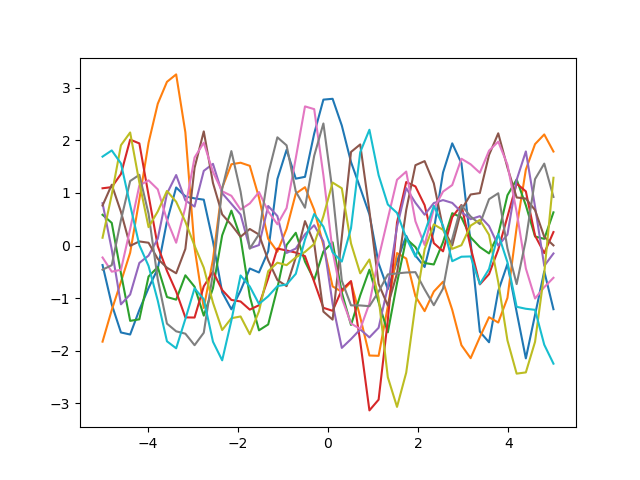
\includegraphics[width=0.5\textwidth]{10prior}
\end{figure}

Običajno nas ne zanimajo naključne funkcije iz apriorija, ampak želimo vključiti znanje o funkciji, ki ga zagotavljajo vhodni učni podatki.
Najprej bomo obravnavali preprost poseben primer, kjer bodo opazovanja brez šuma, 
torej $ \{ (x_{i}, f_{i}) | i = 1, \ldots , n\}$.

Skupna porazdelitev učnih izhodov $f$ in testnih izhodov $f_{*}$, glede na apriori je
\begin{equation}
\begin{bmatrix}
f\\ 
f_{*}
\end{bmatrix}
\sim \mathcal{N} ( 0, 
\begin{bmatrix}
K(X,X) & K(X,X_{*}) \\ 
K(X_{*},X) & K(X_{*},X_{*})
\end{bmatrix})
\end{equation}

Če imamo $n$ učnih točk in $n_{*}$ testnih točk, je $K(X, X_{*})$ $ n \times n_{*}$ matrika
kovarianc vseh parov učnih in testnih točk. 

Da dobimo posteriorno porazdelitev funkcij, moramo omejiti skupno apriori porazdelitev tako, 
da bo vsebovala le funkcije, ki se prilegajo oz. vsebujejo opazovane vhodne točke. 

\opomba Če bi posteriori funckije generirali kar iz apriori funkcij in potem odstranjevali tiste, ki se prilegajo vhodnim točkam, 
bi metoda sicer delovala, vendar bi bila računsko zelo zahtevna. 

\begin{izrek}\label{izrek2} Naj je $ \begin{bmatrix}
x\\ 
y
\end{bmatrix} $ normalno porazdeljen vektor
\begin{equation}
 \begin{bmatrix}
x\\ 
y
\end{bmatrix} \sim \mathcal{N}(\begin{bmatrix}
\mu_{x}\\ 
\mu_{y}
\end{bmatrix}, \begin{bmatrix}
A & C\\ 
C^\top & B
\end{bmatrix}) 
\end{equation}
potem sta \textbf{robna} porazdelitev $x$ in \textbf{pogojna} porazdelitev $x$ glede na $y$ enaki

\begin{equation}
\begin{split}
& x \sim \mathcal{N} (\mu_{x}, A) \\
& x|y \sim \mathcal{N} (\mu_{x} + CB^{-1}(y-\mu_{y}), A-CB^{-1}C^\top).
\end{split}
\end{equation}
\end{izrek}


Če upoštevamo izrek \ref{izrek2} dobimo porazdelitev posteriori funkcij

\begin{equation}
\begin{split}
f_{*} |( X_{*}, X, f ) ~ \sim ~ \mathcal{N} ( &K(X_{*},X) K(X,X)^{-1} f, \\
& K(X_{*},X_{*}) - K(X_{*},X)K(X,X)^{-1}K(X,X_{*})).
\end{split}
\end{equation}

Vrednosti funkcije $f_{*}$ dobimo s pomočjo prej opisanega postopka. 

\begin{figure}[h]
\caption{Primer 10 naključnih funkcij iz GP posterior}
\centering
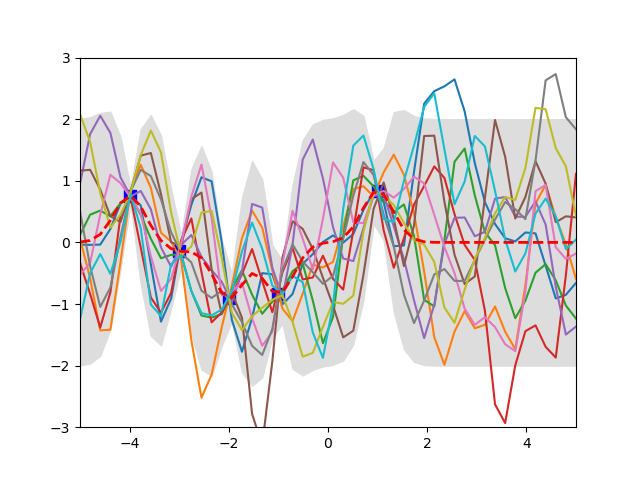
\includegraphics[width=0.5\textwidth]{10posterior}
\end{figure}

\opomba Slika 2 prikazuje rezultate teh izračunov na petih danih točkah označenih z modrim + simbolom. 
Očitno se da te izračune opraviti tudi na več dimenzionalnih podatkih, vendar je funkcije, ki jih dobimo, težje grafično prikazati.


\section{Kovariančne funkcije}
Vloga kovariančne funkcije je pri modeliranju z Gaussovimi procesi zelo pomembna. Napovedane verjetnostne porazdelitve, ki nastopajo pri danih podatkih, so v glavnem odvisne od kovariančne funkcije in njenih hiperparametrov.
Kovariančna funkcija $C(x_{i}, x_{j})$ izraža mero podobnosti med vhodoma $x_{i}$ in $x_{j}$. Za realne procese je navadno sestavljena iz dveh delov:
\begin{equation}
C(x_{i}, x_{j}) = C_{f}(x_{i}, x_{j}) + C_{n}(x_{i}, x_{j})
\end{equation}

Prvi, tj. funkcijski de $C_{f}(x_{i}, x_{j})$, opisuje lastnosti neznanega sistema, ki ga želimo modelirati, drugi, šumni del $C_{n}(x_{i}, x_{j})$ pa predstavlja varianco šuma. Pogosto predpostavljamo, da je šum naključen, kar pomeni, da ne pričakujemo korelacije med šumom in določenimi izhodi. Kovariančne funkcije delimo na stacionarne in nestacionarne. 

\subsection{Stacionarne kovariančne funkcije}
 
Stacionarne kovariančne funkcije $C_{f}(x_{i}, x_{j})$ so tiste, pri katerih je vrednost funkcije odvisna samo od relativne lege vhodnih vektorjev $x_{i}$ in $x_{j}$ oz. od njune medsebojne razdalje $ r= | x_{i} - x_{j} |$. 

Najpreprostejša oblika kovariančne funkcije je konstantna kovariančna funkcija, ki zavazame isto vrednost na celotnem območju. Opišemo jo z izrazom
\begin{equation}
C_{f}(r) = \frac{1}{\theta_{1}^2}
\end{equation}
Določena je z enim hiperparametrom $\theta_{1}$, ki predstavlja skalirni faktor variance učnih podatkov.


% slovar
\section*{Slovar strokovnih izrazov}

%\geslo{}{}
%
%\geslo{}{}
%


% seznam uporabljene literature
\begin{thebibliography}{99}

\bibitem{}http://valjhun.fmf.uni-lj.si/$\sim$raicm/Vaje/BPSt/Verjetnost\_os.pdf

\end{thebibliography}

\end{document}

